\chapter{Run~3 L1Calo $E^{miss}_{T}$ Trigger Optimization}
The $E^{miss}_{T}$ trigger was optimized by scanning through possible $E_T$ cuts of LAr, tile, and forward jTowers. The scan was performed by the steps of $0.5\sigma$ ranged from 0 to $6\sigma$ for LAr and tile jTowers, while the forward towers have threshold higher than LAr tower one ranged from 0 to $2.5\sigma$. The result is shown in Fig.~\ref{Fig:met_optimize}.
\begin{figure}[ht]
	\centering
	\subfloat[]{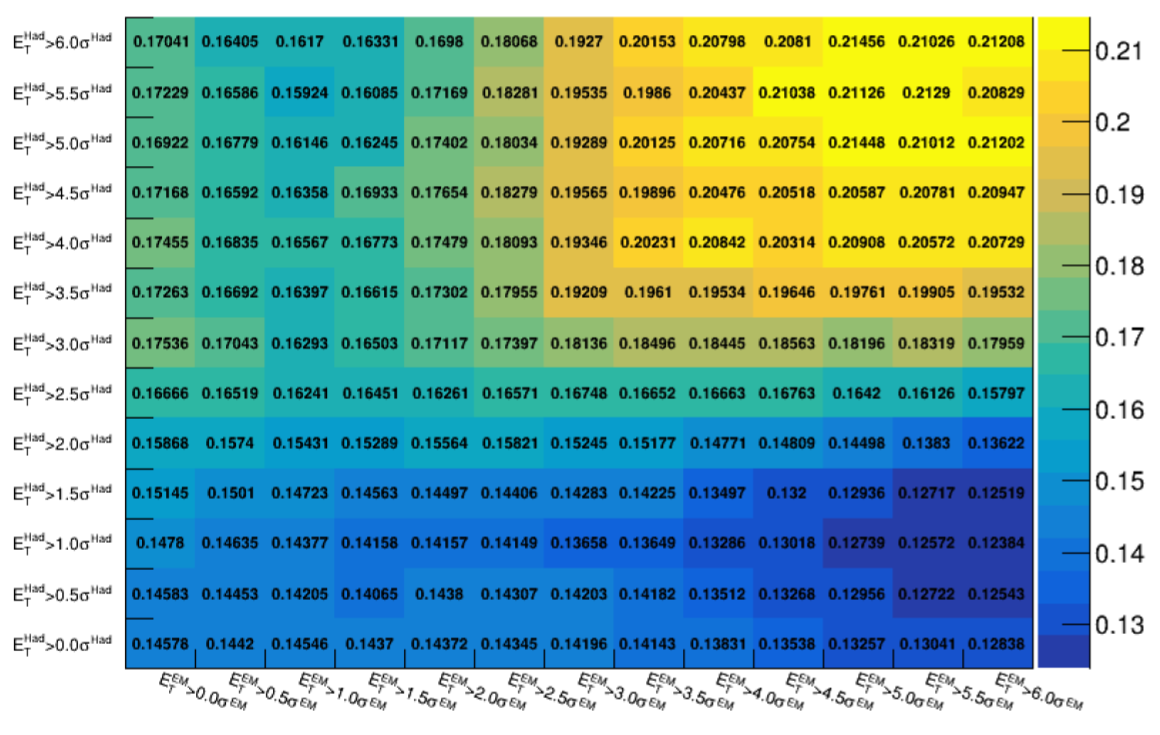
\includegraphics[width=0.4\textwidth]{Chapter6/efficiency_5kHz_cfg0}}
	\subfloat[]{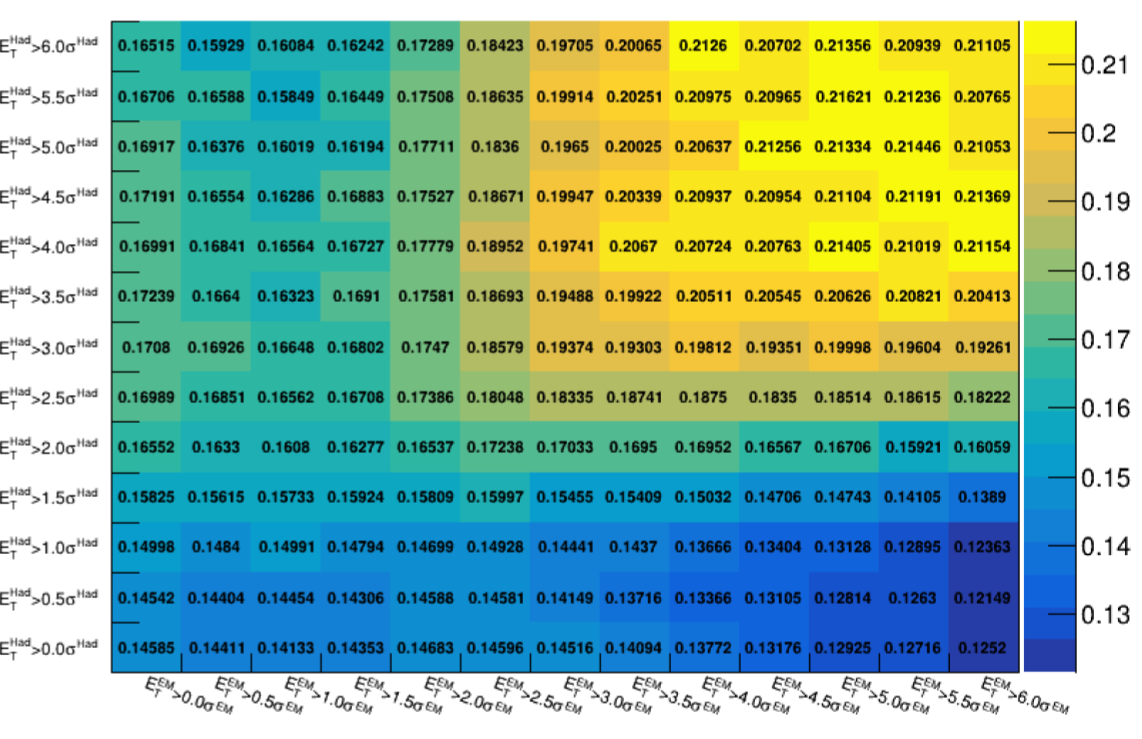
\includegraphics[width=0.4\textwidth]{Chapter6/efficiency_5kHz_cfg1}}\\
	\subfloat[]{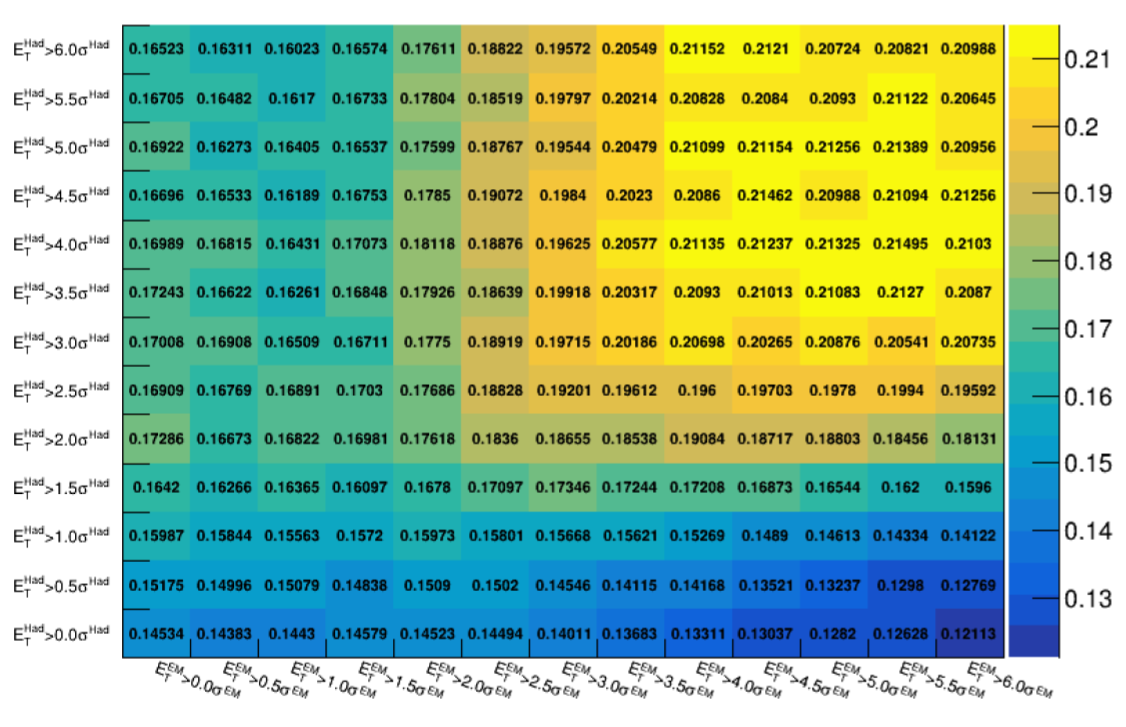
\includegraphics[width=0.4\textwidth]{Chapter6/efficiency_5kHz_cfg2}}
	\subfloat[]{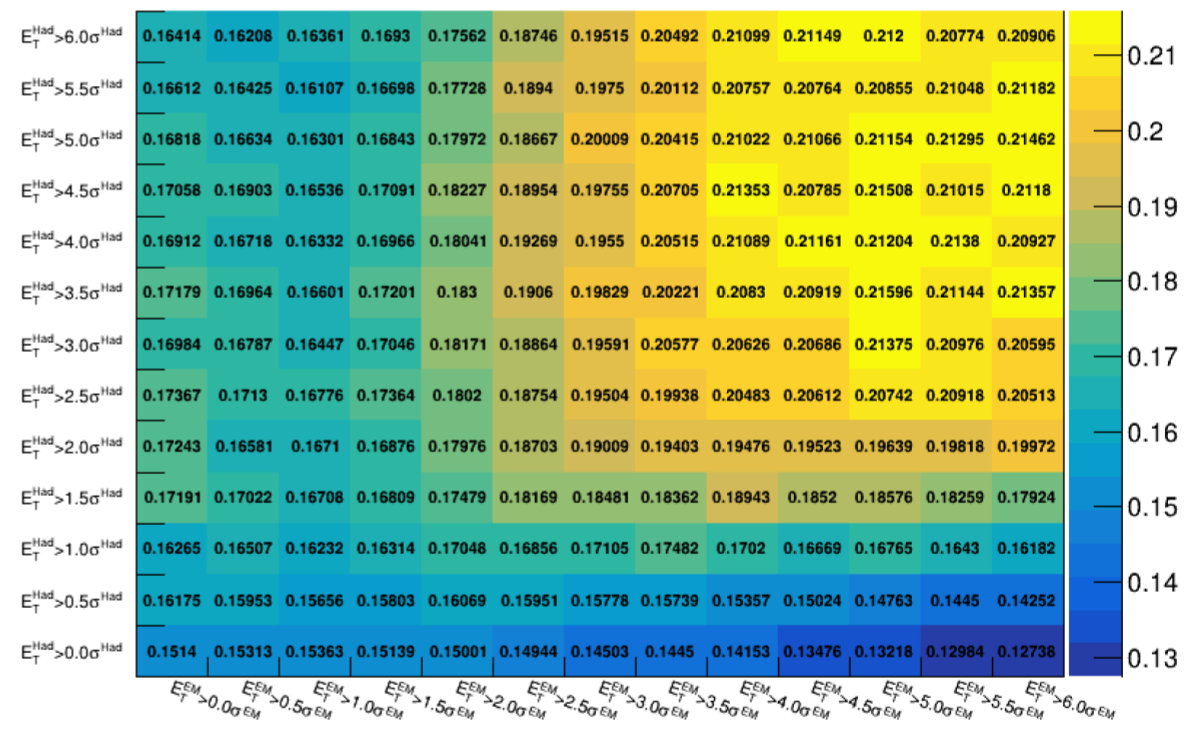
\includegraphics[width=0.4\textwidth]{Chapter6/efficiency_5kHz_cfg3}}\\
	\subfloat[]{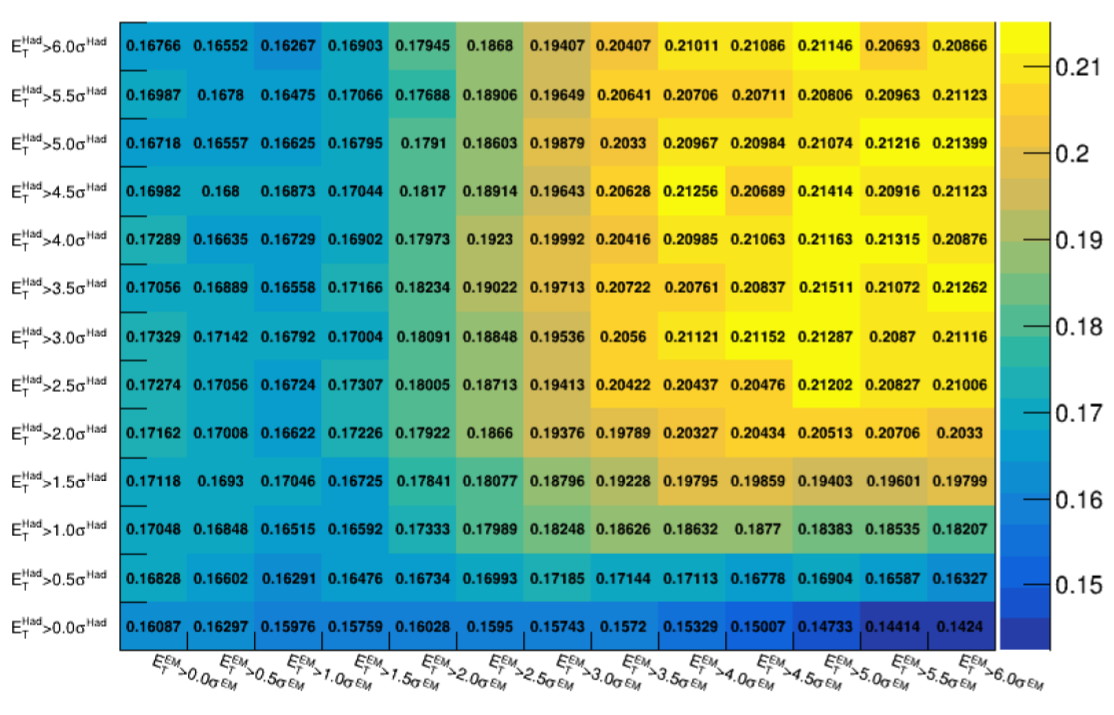
\includegraphics[width=0.4\textwidth]{Chapter6/efficiency_5kHz_cfg4}}
	\subfloat[]{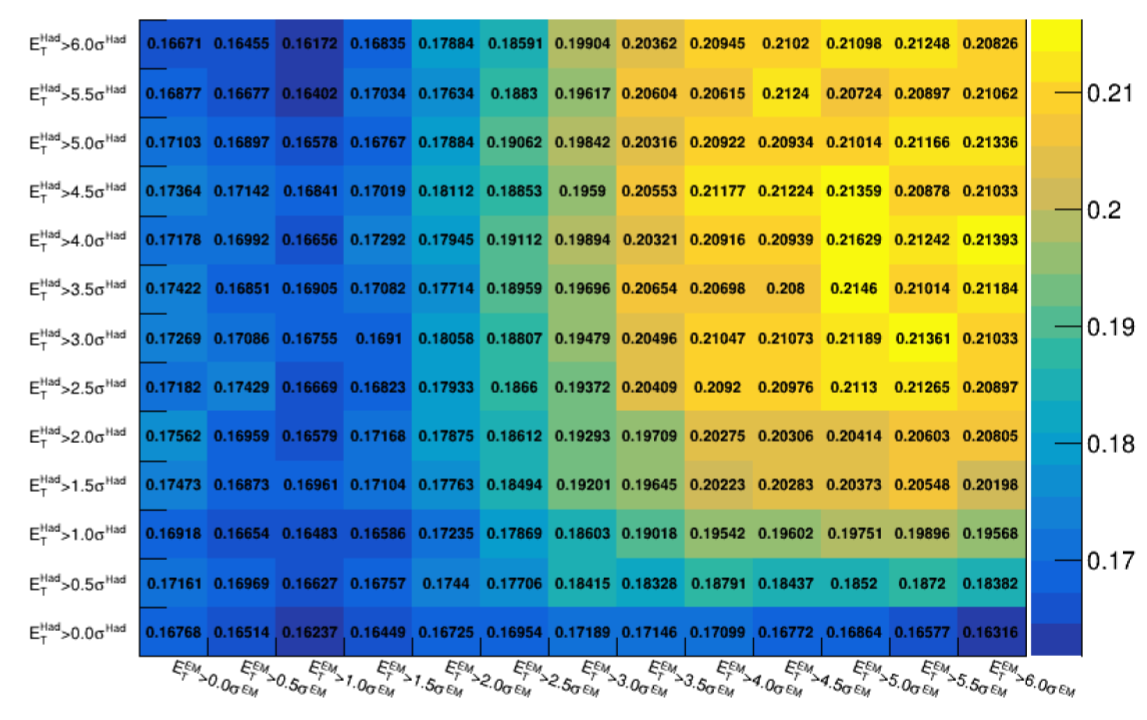
\includegraphics[width=0.4\textwidth]{Chapter6/efficiency_5kHz_cfg5}}
	\caption{The $E^{miss}_{T}$ trigger signal efficiency with different thresholds on jTowers, when the trigger rate is 5~kHz. The six figures presents different threshold in the forward region: (a) $0\sigma$, (b) $0.5\sigma$, (c) $1.0\sigma$, (d) $1.5\sigma$, (e) $2.0\sigma$, and (f)  $2.5\sigma$ higher than the LAr jTower $E_{T}$ thresholds}
	\label{Fig:met_optimize}
\end{figure}

\chapter{Supercells in the ATLAS Forward Region}
Here shows the supercell layouts in the forward region. They are in irregular shapes, so the supercell to j/gTower mapping has a complicated scheme. 
\begin{figure}[ht]
	\centering
    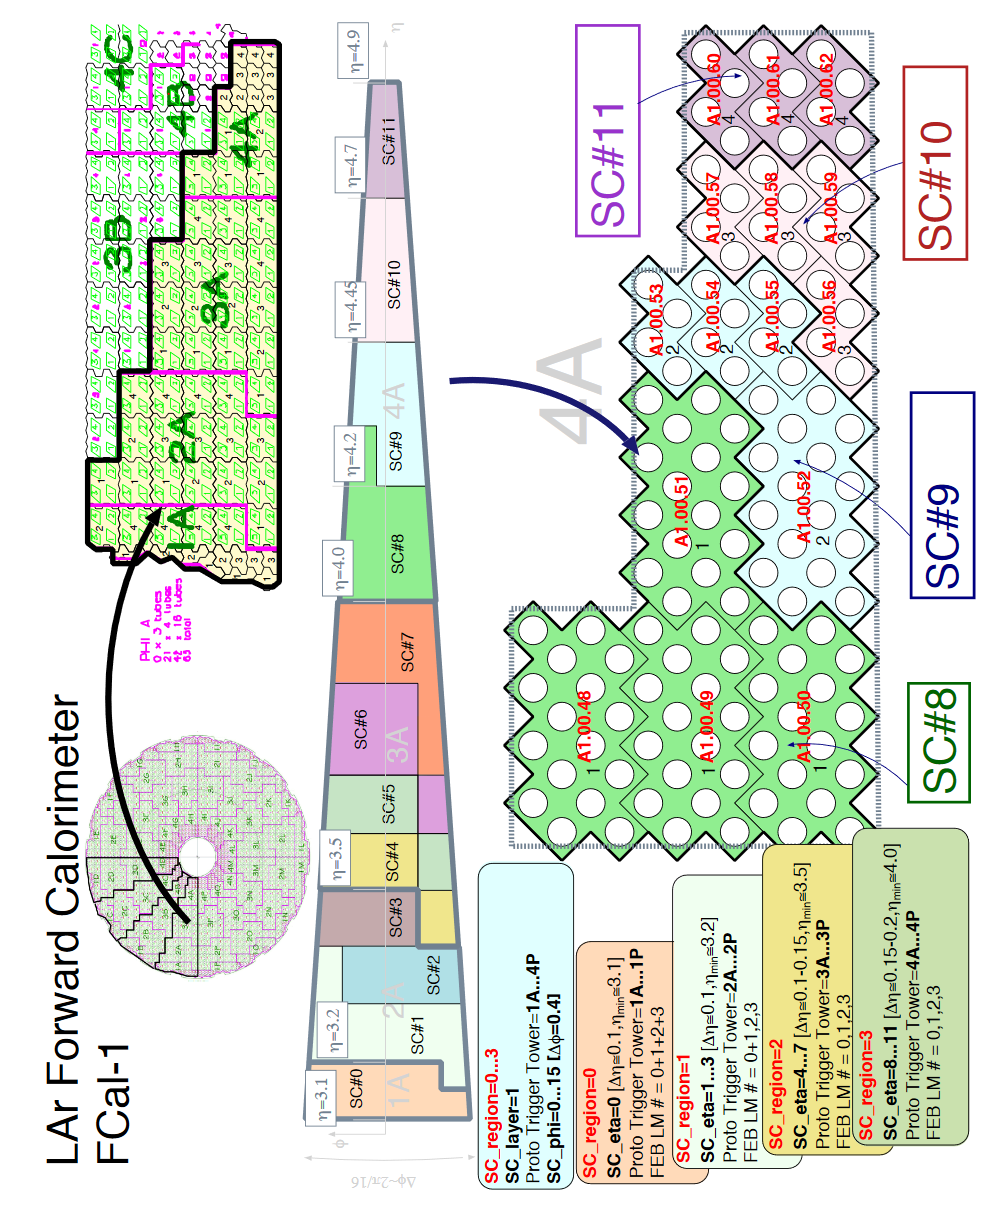
\includegraphics[width=0.95\textwidth]{Chapter6/FCAL1.png}
	\caption{The front layer of the forward LAr detector}
\end{figure}
\begin{figure}[ht]
	\centering
	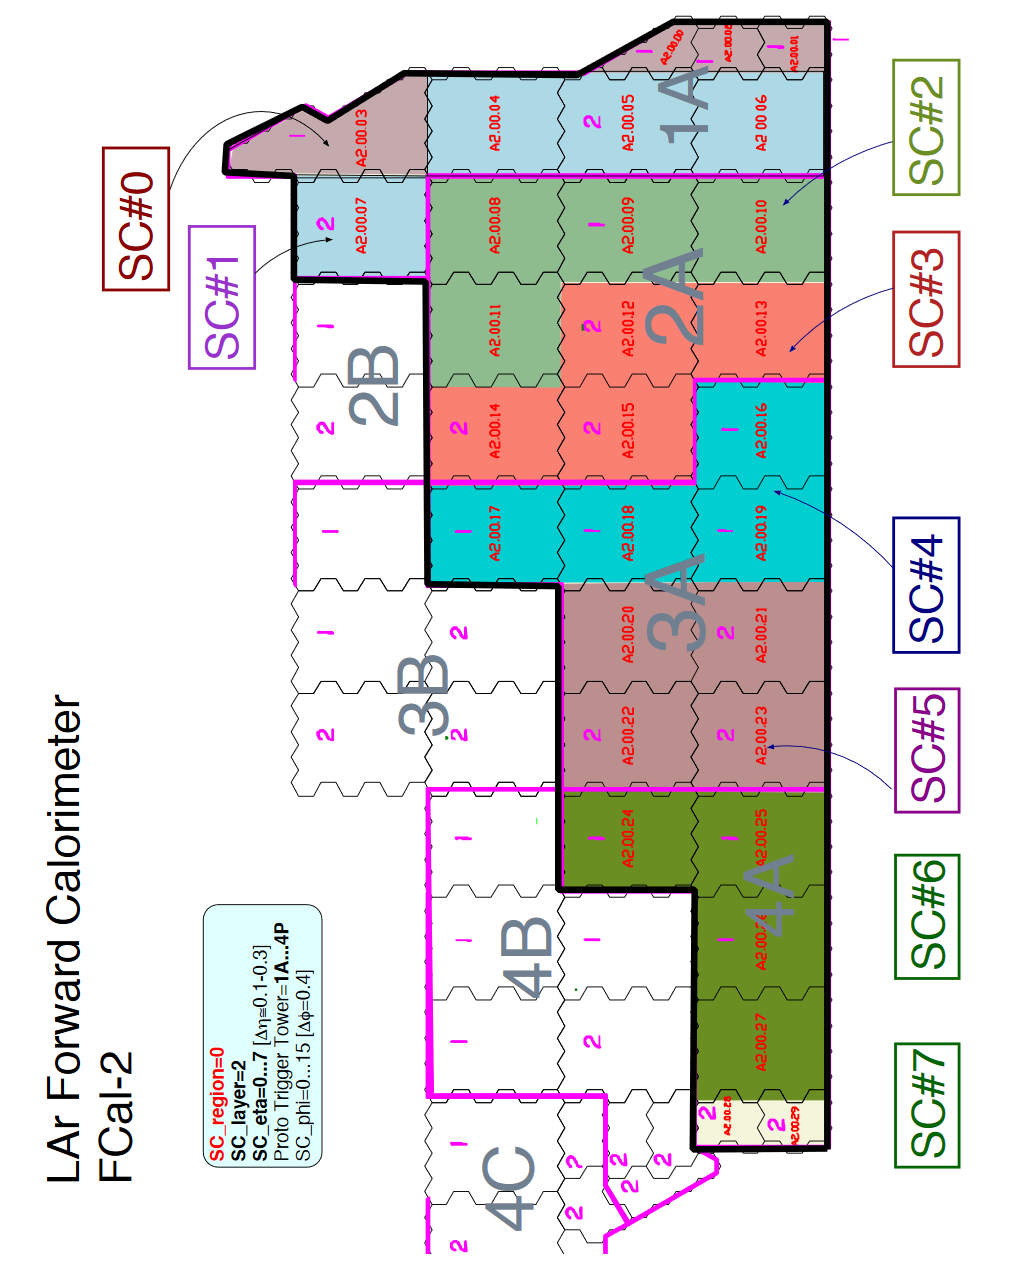
\includegraphics[width=0.95\textwidth]{Chapter6/FCAL2.png}
	\caption{The middle layer of the forward LAr detector}
\end{figure}
\begin{figure}[ht]
	\centering
	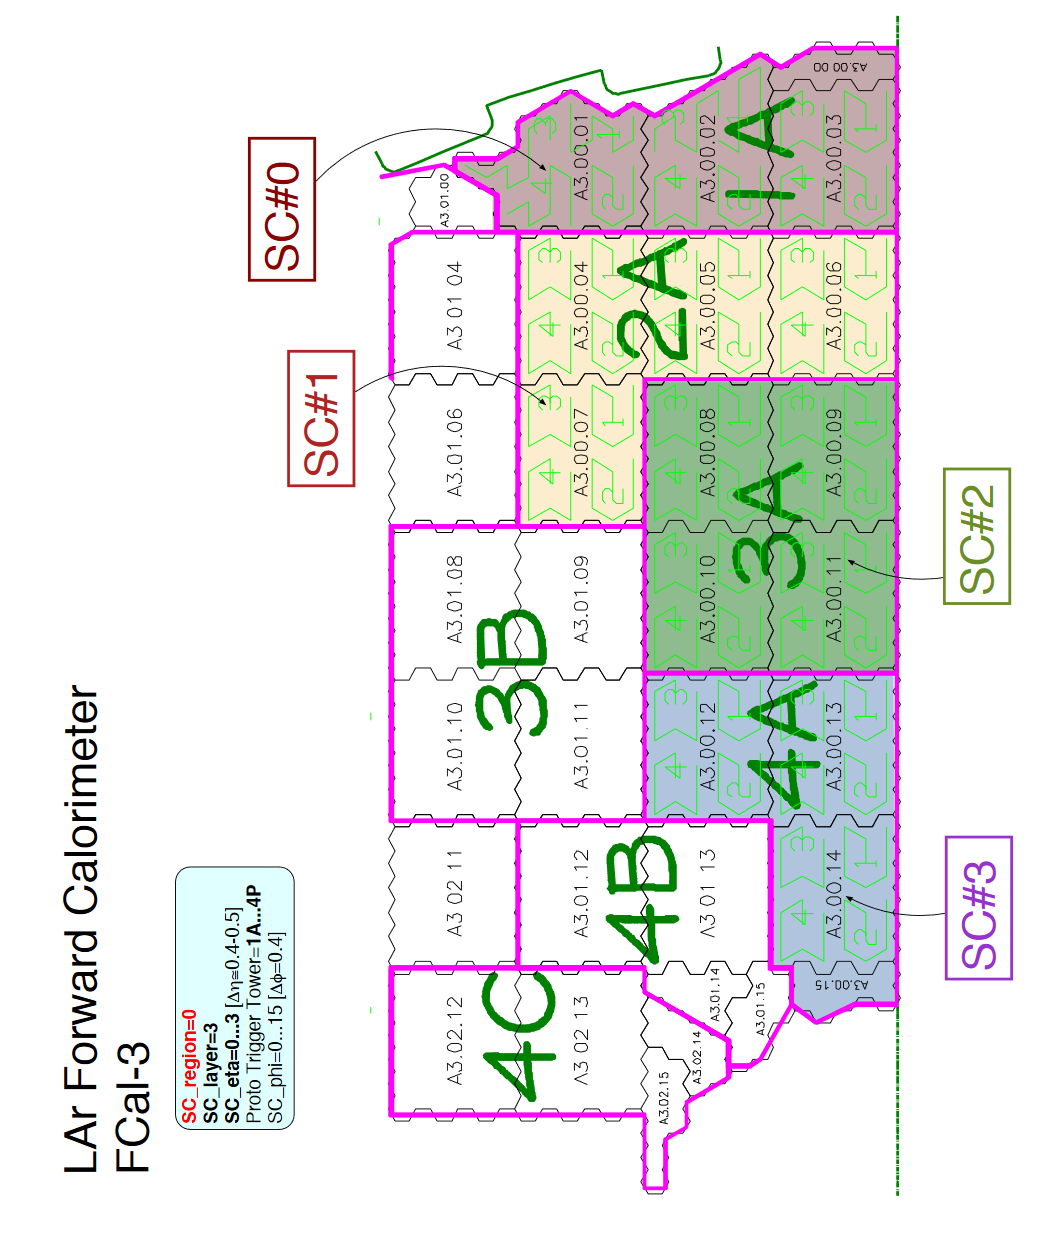
\includegraphics[width=0.95\textwidth]{Chapter6/FCAL3.png}
	\caption{The back layer of the forward LAr detector}
\end{figure}